\begin{figure}[!ht]
    \centering
    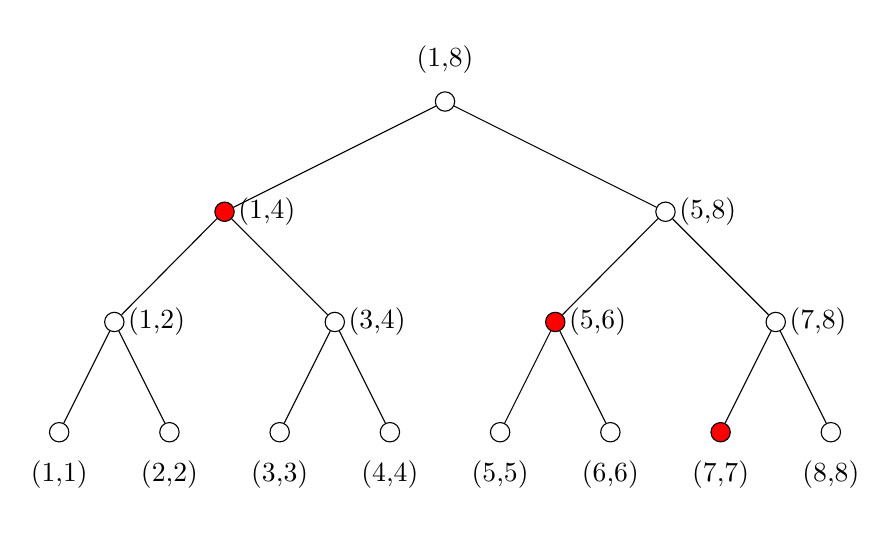
\begin{tikzpicture}[
    level 1/.style={sibling distance=56mm},
    level 2/.style={sibling distance=28mm},
    level 3/.style={sibling distance=14mm},
    level distance=14mm,
    every node/.style={
        circle,
        draw,
        minimum size=7pt,
        inner sep=0pt,
    },
    edge from parent/.style={draw, -},
    ]
    \node[label=above:{\mbox{(1,8)}}] {}
        child {
            node[label=east:{\mbox{(1,4)}},fill=red] {}
            child {
                node[label=east:{\mbox{(1,2)}}] {}
                child { node[label=below:{(1,1)}] {} }
                child { node[label=below:{(2,2)}] {} }
            }
            child {
                node[label=east:{\mbox{(3,4)}}] {}
                child { node[label=below:{(3,3)}] {} }
                child { node[label=below:{(4,4)}] {} }
            }
        }
        child {
            node[label=east:{\mbox{(5,8)}}] {}
            child {
                node[label=east:{\mbox{(5,6)}},fill=red] {}
                child { node[label=below:{(5,5)}] {} }
                child { node[label=below:{(6,6)}] {} }
            }
            child {
                node[label=east:{\mbox{(7,8)}}] {}
                child { node[label=below:{(7,7)},fill=red] {} }
                child { node[label=below:{(8,8)}] {} }
            }
        };
    \end{tikzpicture}
    \caption{An illustration of the {\tree} mechanism using a binary tree. For $n=7$, $\mathsc{Node}(7)=\{4,6,7\}$ and $\tree(7)=\vecr_4 + \vecr_6 + \vecr_7$ with a total noise of order $O(\log(n))$.}
    \label{fig:tree-illustration}
\end{figure}
